\documentclass[11pt,a4paper]{article}

% ── Geometry ──────────────────────────────────────────────────────────────────
\usepackage[top=2cm,bottom=2cm,left=2cm,right=2cm,headheight=14pt]{geometry}

% ── Encoding & fonts ──────────────────────────────────────────────────────────
\usepackage[T1]{fontenc}
\usepackage[utf8]{inputenc}
\usepackage{lmodern}

% ── Colors (Muted Tones) ──────────────────────────────────────────────────────
\usepackage{xcolor}
\definecolor{MainBlack}{HTML}{222222}
\definecolor{DimGray}{HTML}{666666}
\definecolor{ToneGrayBg}{HTML}{F5F5F5}
\definecolor{ToneGrayFrame}{HTML}{333333}
\definecolor{ToneBlueBg}{HTML}{F0F7FF}
\definecolor{ToneBlueFrame}{HTML}{2E5A88}
\definecolor{ToneRedBg}{HTML}{FFF5F5}
\definecolor{ToneRedFrame}{HTML}{A33333}

\definecolor{AxisRed}{HTML}{C8102E}
\definecolor{AxisBlue}{HTML}{1A5276}
\definecolor{AxisGreen}{HTML}{1D8348}

% ── Math & Units ──────────────────────────────────────────────────────────────
\usepackage{amsmath}
\usepackage{siunitx}
\sisetup{
  per-mode = symbol,
  range-phrase = { to },
  range-units = single,
}

% ── Tables ────────────────────────────────────────────────────────────────────
\usepackage{booktabs}
\usepackage{array}
\usepackage{tabularx}
\usepackage[table]{xcolor}

% ── Code listings ─────────────────────────────────────────────────────────────
\usepackage{listings}

\lstdefinestyle{PythonStyle}{
  language=Python,
  basicstyle=\ttfamily\small,
  keywordstyle=\bfseries,
  commentstyle=\color{DimGray}\itshape,
  stringstyle=\color{DimGray},
  numberstyle=\tiny\color{DimGray},
  backgroundcolor=\color{ToneGrayBg},
  frame=single,
  rulecolor=\color{ToneGrayFrame!20},
  breaklines=true,
  tabsize=4,
  showstringspaces=false,
  xleftmargin=5pt,
}

\lstdefinestyle{BashStyle}{
  language=bash,
  basicstyle=\ttfamily\small,
  keywordstyle=\bfseries,
  backgroundcolor=\color{black!5},
  frame=leftline,
  framerule=2pt,
  rulecolor=\color{ToneGrayFrame},
  numbers=none,
  breaklines=true,
  tabsize=4,
  showstringspaces=false,
  xleftmargin=10pt,
}

% ── Modern Boxes (Accent Style) ───────────────────────────────────────────────
\usepackage[most]{tcolorbox}

\tcbset{
  accentbox/.style={
    enhanced,
    breakable,
    sharp corners,
    boxrule=0pt,
    leftrule=3pt,
    left=10pt, right=10pt, top=8pt, bottom=8pt,
    fonttitle=\bfseries\small,
    attach title to upper,
    after title={\par\smallskip\hrule\smallskip},
  },
  setupbox/.style={
    accentbox,
    colback=ToneGrayBg,
    colframe=ToneGrayFrame,
    coltitle=ToneGrayFrame,
  },
  safetybox/.style={
    accentbox,
    colback=ToneRedBg,
    colframe=ToneRedFrame,
    coltitle=ToneRedFrame,
  },
  infobox/.style={
    accentbox,
    colback=ToneBlueBg,
    colframe=ToneBlueFrame,
    coltitle=ToneBlueFrame,
  },
  outcomebox/.style={
    accentbox,
    colback=white,
    colframe=MainBlack,
    coltitle=MainBlack,
    title={Lab Outcomes},
  },
}

% ── Lists ─────────────────────────────────────────────────────────────────────
\usepackage{enumitem}
\setlist{noitemsep, topsep=3pt}

% ── TikZ ──────────────────────────────────────────────────────────────────────
\usepackage{tikz}
\usetikzlibrary{arrows.meta, calc}

% ── Headers & footers ─────────────────────────────────────────────────────────
\usepackage{fancyhdr}
\pagestyle{fancy}
\fancyhf{}
\renewcommand{\headrulewidth}{0.4pt}
\renewcommand{\footrulewidth}{0.4pt}
\lhead{\textbf{ME403 -- Introduction to Robotics}}
\rhead{\textit{Lab 00: Introduction Week}}
\lfoot{\small Sabanci University, Spring 2025-26}
\rfoot{\small Page \thepage}

% ── Section formatting ────────────────────────────────────────────────────────
\usepackage{titlesec}
\titleformat{\section}
  {\large\bfseries}
  {\thesection.}{0.5em}{}
  [\rule{\linewidth}{0.8pt}]

\titleformat{\subsection}
  {\normalsize\bfseries}
  {\thesubsection.}{0.5em}{}

\titlespacing*{\section}{0pt}{18pt}{8pt}
\titlespacing*{\subsection}{0pt}{12pt}{6pt}

% ── Hyperlinks ────────────────────────────────────────────────────────────────
\usepackage{hyperref}
\hypersetup{
  colorlinks=true,
  linkcolor=MainBlack,
  urlcolor=ToneBlueFrame,
  citecolor=MainBlack,
}

% ── Misc ──────────────────────────────────────────────────────────────────────
\setlength{\parskip}{6pt}
\setlength{\parindent}{0pt}

% ──────────────────────────────────────────────────────────────────────────────
\begin{document}

% ── Title block ───────────────────────────────────────────────────────────────
\thispagestyle{fancy}
\begin{center}
  \rule{\linewidth}{1.5pt}\\[8pt]
  {\LARGE\bfseries ME403 -- Introduction to Robotics}\\[4pt]
  {\large\bfseries Lab 00: Introduction Week Handout}\\[4pt]
  {\normalsize Sabanci University \quad|\quad Spring 2025-26}\\[4pt]
  {\small Prepared by Yunus Emre Danabas for ME403}\\[6pt]
  \rule{\linewidth}{1.5pt}
\end{center}

\vspace{5pt}

\begin{tcolorbox}[outcomebox]
  By the end of this lab, you will be able to:
  \begin{itemize}
    \item Configure a Python environment for robotic control using Mamba or venv.
    \item Establish and verify communication with both Magician (Serial) and MG400 (TCP/IP).
    \item Understand the relationship between relative and absolute joint angles.
    \item Manually calculate and verify Forward Kinematics (FK) for a 4-axis arm.
  \end{itemize}
\end{tcolorbox}

% ──────────────────────────────────────────────────────────────────────────────
\section{Overview}
% ──────────────────────────────────────────────────────────────────────────────

This lab session focuses on setting up your development environment and verifying the connection with your assigned robotic arm. The lab supports two robots: the \textbf{Dobot Magician} (USB-serial) and the \textbf{DOBOT MG400} (TCP/IP over Ethernet). Scripts are organized into separate folders — \texttt{magician/} and \texttt{mg400/}.

\subsection*{Included Scripts}

\renewcommand{\arraystretch}{1.5}
\begin{tabularx}{\linewidth}{@{}lX@{}}
  \toprule
  \textbf{Script} & \textbf{Purpose} \\
  \midrule
  \multicolumn{2}{@{}l@{}}{\textit{Dobot Magician (\texttt{magician/})}} \\
  \texttt{01\_init\_check.py} & Verifies USB connection, clears alarms, and moves to safe ready pose. Run first. \\
  \texttt{02\_joint\_control.py} & Interactive REPL: enter joint angles in degrees to move joints. \\
  \texttt{03\_relative\_joint\_control.py} & Body-frame FK exercise: enter relative joint angles, observe the conversion chain. \\
  \midrule
  \multicolumn{2}{@{}l@{}}{\textit{DOBOT MG400 (\texttt{mg400/})}} \\
  \texttt{01\_init\_check.py} & Verifies Ethernet connection, enables robot, moves to \texttt{READY\_POSE}. \\
  \texttt{02\_joint\_control.py} & Interactive REPL: enter joint angles with FK preview and joint clamping. \\
  \texttt{03\_relative\_joint\_control.py} & Body-frame FK exercise: enter relative joint angles, observe conversion and prediction. \\
  \bottomrule
\end{tabularx}

% ──────────────────────────────────────────────────────────────────────────────
\section{Quick Start Guide}
% ──────────────────────────────────────────────────────────────────────────────

\subsection{Dobot Magician (USB-serial)}

\begin{tcolorbox}[setupbox, title={Magician — Mamba (Recommended)}]
\begin{lstlisting}[style=BashStyle]
# 1. Activate environment and install
mamba activate dobot
pip install -r magician/requirements.txt

# 2. Verify connection
cd magician
python 01_init_check.py
\end{lstlisting}
\end{tcolorbox}

\begin{tcolorbox}[setupbox, title={Magician — Python venv}]
\begin{lstlisting}[style=BashStyle]
python3 -m venv .venv
source .venv/bin/activate    # Linux/macOS
# .venv\Scripts\activate     # Windows
pip install -r magician/requirements.txt
cd magician && python 01_init_check.py
\end{lstlisting}
\end{tcolorbox}

\subsection{DOBOT MG400 (Ethernet/TCP-IP)}

\begin{tcolorbox}[setupbox, title={MG400 — One-time SDK Setup}]
\begin{lstlisting}[style=BashStyle]
# Clone the official Dobot SDK into the vendor/ directory
cd dobot_ws
git clone https://github.com/Dobot-Arm/TCP-IP-4Axis-Python.git \
    vendor/TCP-IP-4Axis-Python
# Set PC Ethernet to static IP 192.168.2.100 / 255.255.255.0
# Verify: ping 192.168.2.9
\end{lstlisting}
\end{tcolorbox}

\begin{tcolorbox}[setupbox, title={MG400 — Run Scripts}]
\begin{lstlisting}[style=BashStyle]
pip install -r mg400/requirements.txt

# Default: Robot 1 (192.168.2.9)
cd mg400 && python 01_init_check.py

# Select a specific robot (1-4)
python 01_init_check.py --robot 2
\end{lstlisting}
\end{tcolorbox}

% ──────────────────────────────────────────────────────────────────────────────
\section{Hardware Configuration}
% ──────────────────────────────────────────────────────────────────────────────

\subsection{Dobot Magician (USB-serial)}

\begin{enumerate}
  \item \textbf{Surface:} Place on a flat, stable surface. Clear a \qty{40}{\cm} radius around the base.
  \item \textbf{Posture:} Manually set the arm to a neutral posture (both segments at $\approx$\qty{45}{\degree}) before powering on.
  \item \textbf{Power:} Connect the \qty{12}{\V} DC adapter. \textbf{USB power alone is insufficient.}
  \item \textbf{Communication:} Connect the USB cable (CP210x USB-to-UART bridge).
\end{enumerate}

\textbf{Status Signals:}
\begin{itemize}
  \item \textbf{Green LED + Single Beep:} Ready.
  \item \textbf{Red LED + Rapid Beeping:} Alarm state — run \texttt{01\_init\_check.py} to clear.
  \item \textbf{Yellow/Flashing LED:} Busy (homing or executing a command).
\end{itemize}

\subsection{DOBOT MG400 (Ethernet/TCP-IP)}

\begin{enumerate}
  \item \textbf{Surface:} Place on a flat, stable surface. Clear a \qty{50}{\cm} radius around the base (\qty{440}{\mm} reach).
  \item \textbf{Power:} Connect the DC power adapter. Wait for the status LED to turn solid green.
  \item \textbf{Network:} Connect an Ethernet cable from the robot to your PC.
  \item \textbf{PC Static IP:} Set your Ethernet adapter to \texttt{192.168.2.100}, netmask \texttt{255.255.255.0}.
  \item \textbf{Verify:} \texttt{ping 192.168.2.9} — should respond with $<$\qty{1}{\ms} latency.
\end{enumerate}

\textbf{Robot IP addresses (192.168.2.x subnet):}

\begin{tabularx}{0.8\linewidth}{@{}llX@{}}
  \toprule
  \textbf{Robot} & \textbf{IP Address} & \textbf{CLI flag} \\
  \midrule
  1 & 192.168.2.9  & \texttt{--robot 1} (default) \\
  2 & 192.168.2.10 & \texttt{--robot 2} \\
  3 & 192.168.2.7  & \texttt{--robot 3} \\
  4 & 192.168.2.8  & \texttt{--robot 4} \\
  \bottomrule
\end{tabularx}

% ──────────────────────────────────────────────────────────────────────────────
\section{Software and OS Setup}
% ──────────────────────────────────────────────────────────────────────────────

\subsection{Linux Setup (Dobot Magician only)}
Users must have permission to access serial devices. Run the following once:
\begin{lstlisting}[style=BashStyle]
sudo usermod -a -G dialout $USER
# Log out and log back in for changes to take effect.
\end{lstlisting}
The Magician typically appears as \texttt{/dev/ttyUSB0} or \texttt{/dev/ttyACM0}.
The MG400 uses Ethernet (no serial permission needed).

\subsection{Windows Setup}
The driver is usually handled by Windows Update. To find the port:
\begin{enumerate}
  \item Open \textbf{Device Manager}.
  \item Expand \textbf{Ports (COM \& LPT)}.
  \item Look for \textbf{Silicon Labs CP210x USB to UART Bridge} (e.g., \texttt{COM3}).
\end{enumerate}

\subsection{macOS Setup}
Modern macOS versions include the driver. The device will appear as:
\texttt{/dev/cu.usbserial-*} or \texttt{/dev/cu.SLAB\_USBtoUART}.

% ──────────────────────────────────────────────────────────────────────────────
\section{Dobot Magician Reference (USB-serial)}
% ──────────────────────────────────────────────────────────────────────────────

\subsection{Coordinate System (Cartesian)}

\begin{minipage}[t]{0.45\linewidth}
\vspace{0pt}
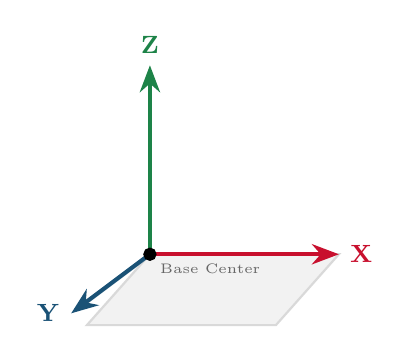
\begin{tikzpicture}[>=Stealth, thick]
  % Grid/Base
  \fill[gray!10] (0,0) -- (2.4,0) -- (1.6,-0.9) -- (-0.8,-0.9) -- cycle;
  \draw[gray!30] (0,0) -- (2.4,0) -- (1.6,-0.9) -- (-0.8,-0.9) -- cycle;
  
  % Axes
  \draw[->, AxisRed, line width=1.5pt] (0,0) -- (2.4,0) node[right]{\small\textbf{X}};
  \draw[->, AxisBlue, line width=1.5pt] (0,0) -- (-1.0,-0.75) node[left]{\small\textbf{Y}};
  \draw[->, AxisGreen, line width=1.5pt] (0,0) -- (0,2.4) node[above, AxisGreen]{\small\textbf{Z}};
  
  % Origin
  \filldraw[black] (0,0) circle (2pt);
  \node[below right, font=\tiny, DimGray] at (0,0) {Base Center};
\end{tikzpicture}
\end{minipage}
\hfill
\begin{minipage}[t]{0.50\linewidth}
\vspace{0pt}
\begin{itemize}
  \item \textbf{\color{AxisRed}X-axis:} Forward (pointing away from base).
  \item \textbf{\color{AxisBlue}Y-axis:} Left/Right (Left is positive).
  \item \textbf{\color{AxisGreen}Z-axis:} Vertical (Up is positive).
  \item \textbf{Units:} Millimeters (\si{\mm}).
  \item \textbf{Rotation (R):} Tool rotation in degrees (\si{\degree}).
\end{itemize}
\end{minipage}

\subsection{Joint Definitions and Safe Limits}

\begin{tabularx}{\linewidth}{@{}llXl@{}}
  \toprule
  \textbf{Joint} & \textbf{Motion} & \textbf{Safe Range} & \textbf{Units} \\
  \midrule
  J1 & Base Rotation & \qtyrange{-90}{90}{\degree} & deg \\
  J2 & Rear Arm Elevation & \qtyrange{0}{85}{\degree} & deg \\
  J3 & Forearm Elevation & \qtyrange{-10}{85}{\degree} & deg \\
  J4 & End-Effector Rotation & \qtyrange{-90}{90}{\degree} & deg \\
  \bottomrule
\end{tabularx}

\vspace{10pt}

\begin{tabularx}{\linewidth}{@{}lXl@{}}
  \toprule
  \textbf{Cartesian Dimension} & \textbf{Safe Operating Range} & \textbf{Unit} \\
  \midrule
  X (Reach) & \qtyrange{120}{315}{\mm} & mm \\
  Y (Slew)  & $\pm$\qty{158}{\mm} & mm \\
  Z (Height) & \qtyrange{5}{155}{\mm} & mm \\
  \bottomrule
\end{tabularx}

% ──────────────────────────────────────────────────────────────────────────────
\section{DOBOT MG400 Reference (Ethernet/TCP-IP)}
% ──────────────────────────────────────────────────────────────────────────────

\subsection{Coordinate System}

The MG400 uses the same X/Y/Z/R convention as the Magician, but with different operating bounds:

\begin{tabularx}{\linewidth}{@{}lXll@{}}
  \toprule
  \textbf{Axis} & \textbf{Safe Range} & \textbf{Unit} & \textbf{Note} \\
  \midrule
  X (Reach)   & \qtyrange{60}{400}{\mm}  & mm  & Inner limit $\approx$\qty{60}{\mm} (singularity) \\
  Y (Slew)    & $\pm$\qty{220}{\mm}   & mm  & Symmetric full lateral sweep \\
  Z (Height)  & \qtyrange{5}{140}{\mm}   & mm  & \textbf{Z cannot go negative} (0\,mm = surface) \\
  R (Rotation) & $\pm$\qty{170}{\degree}  & deg & End-effector wrist rotation \\
  \bottomrule
\end{tabularx}

\vspace{6pt}
\textbf{READY\_POSE} = \texttt{(300, 0, 50, 0)} — safe home position above the surface.

\subsection{Joint Definitions and Limits}

\begin{tabularx}{\linewidth}{@{}llXl@{}}
  \toprule
  \textbf{Joint} & \textbf{Motion} & \textbf{Safe Range} & \textbf{Units} \\
  \midrule
  J1 & Base Rotation      & $\pm$\qty{170}{\degree}              & deg \\
  J2 & Shoulder Elevation & \qtyrange{-5}{90}{\degree} & deg \\
  J3 & Elbow              & \qtyrange{-140}{5}{\degree} & deg \\
  J4 & Wrist Rotation     & $\pm$\qty{170}{\degree}              & deg \\
  \bottomrule
\end{tabularx}

% ──────────────────────────────────────────────────────────────────────────────
\section{Forward Kinematics Exercise (Script 03)}
% ──────────────────────────────────────────────────────────────────────────────

Script \texttt{03\_relative\_joint\_control.py} introduces the concept of
\textbf{body-frame (relative) joint angles} and makes the FK transformation
chain visible in the terminal output.

\subsection{What Are Relative Joint Angles?}

\begin{tcolorbox}[infobox, title={Body-Frame vs.\ World-Frame Angles}]
Each joint angle can be measured from two different reference directions:
\begin{center}
\renewcommand{\arraystretch}{1.4}
\begin{tabularx}{0.95\linewidth}{@{}lXX@{}}
  \toprule
  \textbf{Joint} & \textbf{Relative (body-frame)} & \textbf{Absolute (world-frame)} \\
  \midrule
  J1 & Base rotation from world X-axis & Same as relative \\
  J2 & Shoulder elevation from horizontal & Same as relative \\
  J3 & Elbow offset \textit{from the upper arm} & $= \mathrm{J2} + \mathrm{J3_{rel}}$ \\
  J4 & Wrist offset \textit{from the forearm}   & $= \mathrm{J3_{abs}} + \mathrm{J4_{rel}}$ \\
  \bottomrule
\end{tabularx}
\end{center}
J1 and J2 are identical in both conventions.  J3 and J4 are where they differ:
a relative J3 of \qty{10}{\degree} means the forearm is \qty{10}{\degree} above the upper arm,
regardless of how high the shoulder is.
\end{tcolorbox}

\subsection{Conversion Chain}

The script applies this chain before every move:
\begin{align*}
  j_{3,\text{abs}} &= j_{2,\text{rel}} + j_{3,\text{rel}} \\
  j_{4,\text{abs}} &= j_{3,\text{abs}} + j_{4,\text{rel}}
                    = j_{2,\text{rel}} + j_{3,\text{rel}} + j_{4,\text{rel}}
\end{align*}

\textbf{Magician firmware note:} the Dobot Magician uses a parallel linkage and
its firmware already interprets the J3 channel as a body-frame offset (so
$j_{3,\text{fw}} = j_{3,\text{rel}}$ trivially). Only J4 needs the absolute
wrist angle: $j_{4,\text{fw}} = j_{4,\text{abs}}$.

\textbf{MG400 firmware note:} the MG400 firmware expects fully absolute angles,
so both J3 and J4 must be accumulated: $j_{3,\text{fw}} = j_{3,\text{abs}}$
and $j_{4,\text{fw}} = j_{4,\text{abs}}$.

\subsection{Worked Example (Dobot Magician)}

Input: \texttt{0 20 10 0} (all relative)

\begin{tabularx}{\linewidth}{@{}lX@{}}
  \toprule
  \textbf{Step} & \textbf{Value} \\
  \midrule
  $j_{3,\text{abs}}$ & $= \qty{20}{\degree} + \qty{10}{\degree} = \qty{30}{\degree}$ \\
  $j_{4,\text{abs}}$ & $= \qty{30}{\degree} + \qty{0}{\degree}  = \qty{30}{\degree}$ \\
  $j_{3,\text{fw}}$  & $= \qty{10}{\degree}$ (trivial for Magician) \\
  $j_{4,\text{fw}}$  & $= \qty{30}{\degree}$ (= $j_{4,\text{abs}}$) \\
  FK reach           & $= 135\cos(\qty{20}{\degree})+147\cos(\qty{30}{\degree}) \approx \qty{254}{\mm}$ \\
  FK height          & $= 135\sin(\qty{20}{\degree})+147\sin(\qty{30}{\degree}) \approx \qty{120}{\mm}$ \\
  \bottomrule
\end{tabularx}

\begin{tcolorbox}[safetybox, title={Safety Note}]
Joint bounds are always applied to the \textbf{firmware angles} (absolute),
not the relative inputs.  Entering $j_{3,\text{rel}} = \qty{10}{\degree}$ when
$j_{2,\text{rel}} = \qty{80}{\degree}$ would produce $j_{3,\text{abs}} = \qty{90}{\degree}$,
which exceeds the J3 firmware bound of \qty{85}{\degree} and will be clamped with a
warning before the move executes.
\end{tcolorbox}

\subsection{Usage and Terminal Output}

\begin{lstlisting}[style=BashStyle]
# Dobot Magician
cd magician && python 03_relative_joint_control.py

# DOBOT MG400
cd mg400 && python 03_relative_joint_control.py
python 03_relative_joint_control.py --robot 2
\end{lstlisting}

Sample terminal output for input \texttt{0 20 10 0}:

\begin{lstlisting}[style=BashStyle]
Abs: J1=  0.00  J2= 20.00  J3= 30.00  J4= 30.00
Rel: J1=  0.00  J2= 20.00  J3= 10.00  J4=  0.00
> 0 20 10 0

  Relative:  J1_rel=   0.00  J2_rel=  20.00  J3_rel=  10.00  J4_rel=   0.00
  Absolute:  j1_abs=   0.00  j2_abs=  20.00  j3_abs=  30.00  j4_abs=  30.00
  Firmware:  j1_fw=    0.00  j2_fw=   20.00  j3_fw=   10.00  j4_fw=   30.00
  [FK]       X= 254.17  Y=   0.00  Z= 119.72  R= 30.00
\end{lstlisting}

\textbf{Challenge:} before running the script, calculate the expected X, Y, Z
by hand using the FK formulas. Then compare your answer with the \texttt{[FK]}
line in the terminal.

% ──────────────────────────────────────────────────────────────────────────────
\section{Troubleshooting}
% ──────────────────────────────────────────────────────────────────────────────

\subsection{Dobot Magician}

\begin{tcolorbox}[infobox, title={Magician: Common Connection Issues}]
\rowcolors{2}{white}{ToneBlueBg}
\begin{tabularx}{\linewidth}{@{}lX@{}}
  \toprule
  \textbf{Symptom} & \textbf{Recommended Action} \\
  \midrule
  \texttt{Access Denied} & Ensure \textbf{DobotStudio} and other Python scripts are closed. \\
  \texttt{Device not found} & Verify both USB and Power cables. Check \texttt{ls /dev/tty*} (Unix). \\
  Motors don't move & Check the \qty{12}{\V} supply. If light is red, run \texttt{01\_init\_check.py}. \\
  Erratic movement & Reset to neutral posture and power cycle the robot. \\
  \bottomrule
\end{tabularx}
\end{tcolorbox}

\subsection{DOBOT MG400}

\begin{tcolorbox}[infobox, title={MG400: Common Issues}]
\rowcolors{2}{white}{ToneBlueBg}
\begin{tabularx}{\linewidth}{@{}lX@{}}
  \toprule
  \textbf{Symptom} & \textbf{Recommended Action} \\
  \midrule
  \texttt{dobot\_api.py} missing & Clone the SDK into \texttt{vendor/TCP-IP-4Axis-Python}. \\
  \texttt{Connection refused} & Check Ethernet cable, verify PC IP is \texttt{192.168.2.100}, ping robot. \\
  Robot in ERROR mode & Run \texttt{check\_errors(dashboard)} or press E-stop, release, power-cycle. \\
  Z motion stops early & MG400 Z cannot go negative. Ensure all targets have $Z \geq \qty{5}{\mm}$. \\
  \bottomrule
\end{tabularx}
\end{tcolorbox}

% ──────────────────────────────────────────────────────────────────────────────
\section{Safety Mandates}
% ──────────────────────────────────────────────────────────────────────────────

\begin{tcolorbox}[safetybox, title={Mandatory Safety Rules (Both Robots)}]
\begin{enumerate}
  \item \textbf{Workspace:} Maintain a clean area. No cables in the reach zone (\qty{40}{\cm} for Magician; \qty{50}{\cm} for MG400).
  \item \textbf{Initialization:} Always run \texttt{01\_init\_check.py} before starting your own scripts.
  \item \textbf{Helper Functions:} Use \texttt{safe\_move()} from \texttt{utils.py}. It enforces software limits.
  \item \textbf{Supervision:} Stay within reach of the power cable (or E-stop for MG400).
  \item \textbf{MG400 only:} Z cannot go negative ($Z \geq \qty{5}{\mm}$). Never command below surface.
\end{enumerate}
\end{tcolorbox}

\vfill
\rule{\linewidth}{0.4pt}
\begin{center}
  \small ME403 Introduction to Robotics --- Sabanci University --- Spring 2025-26
\end{center}

\end{document}
